\section{What Recurs: Capacity Association and an Accessible Trainability Residual}
\label{sec:cap-train}
\enlargethispage{-\baselineskip}

\noindent
We read the oriented $29$-proxy zoo (\cref{sec:setup}) one term of the
decomposition lens \cref{eq:decomp} at a time: summarize the zoo by PCA, treat the
leading component as an empirical \emph{capacity} axis, and ask what survives once
capacity $\{\erank,\params\}$ is held fixed against the directly measured
\emph{trainability} target $T$. A scope caveat governs everything below:
Proposition~\ref{thm:bound} prices only the capacity term of \cref{eq:decomp}, and
only for the frozen at-init NTK target, not for the trained accuracy these findings
are about (\cref{sec:setup}). Both axes are analyzed, with sample sizes stated
per analysis: the joined full-zoo cohorts contain $324/138$ rows, whereas the
29-feature PCA-complete cohorts contain $317/138$. Each result traces to a body
exhibit and corresponding appendix evidence (\cref{app:map}).

%-------------------------------------------------------------------------
% CLUSTER SUMMARY BOX (Results 1-4).
%-------------------------------------------------------------------------
\begin{findingframe}
\textbf{Associated structure in the zoo, in brief} (\cref{fig:results}). To first order the
proxy zoo contains a dominant \emph{capacity-associated factor} (PC1 scores track
effective rank and explain ${\sim}$half the variance on both axes), but a
capacity-orthogonal
early-training term ($\partialcorr{\approx}{+}0.6$) remains after capacity
adjustment and is partly predictable at initialization; the axis-specific best
label-free proxies (\px{meco} on TSS, \px{synflow} on SSS) close most of the
observed gap, so no empirical ceiling is detected on these
benchmarks.
\end{findingframe}

\noindent
We summarize above and elaborate next, in the order the findings earn.

%-------------------------------------------------------------------------
% HERO EXHIBIT: the kept 3-panel results figure (covers Results 1-4).
%-------------------------------------------------------------------------
\begin{figure*}[t]
  \centering
  {\small\bfseries
  \makebox[\linewidth][c]{%
    \parbox{0.31\linewidth}{\centering (a) PCA: dominant factor}\hfill
    \parbox{0.34\linewidth}{\centering (b) orientation-sensitive partials}\hfill
    \parbox{0.31\linewidth}{\centering (c) empirical ceiling test}%
  }}
  \vspace{1pt}
  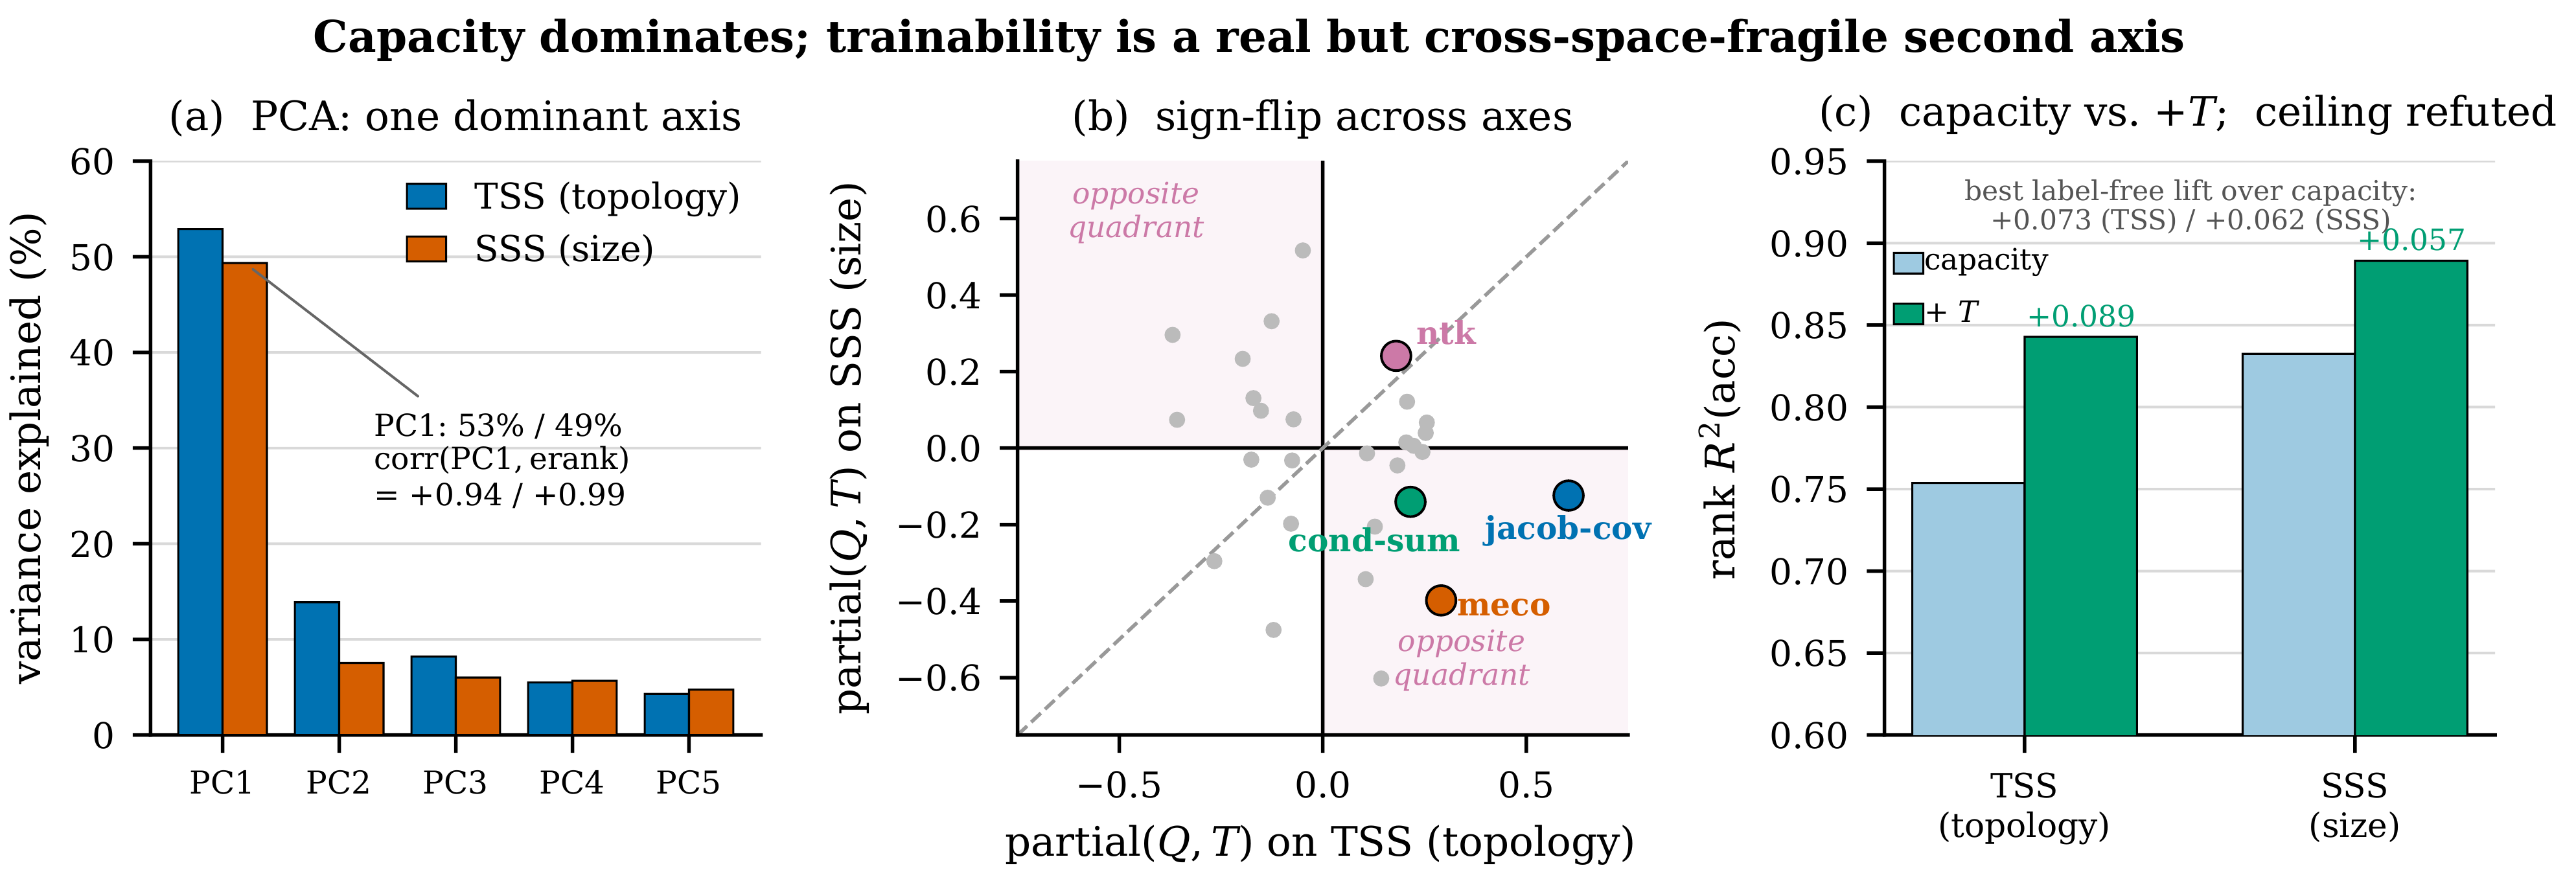
\includegraphics[width=\linewidth,trim=0 0 0 28.5bp,clip]{figures/fig3_results_final.png}
  \caption{\textbf{Capacity is dominant; the early-training association is
  cross-space-fragile.}
  \textbf{(a)} PCA scree of the oriented zoo, PC1 tracking effective rank;
  \textbf{(b)} per-proxy partial $\partialcorr(Q,T\mid\erank,\params)$ on TSS
  ($x$) vs SSS ($y$), opposite-sign quadrants shaded;
  \textbf{(c)} rank-$R^2(\acc)$ of capacity alone vs ${+}$ground-truth $T$ vs
  ${+}$axis-specific best label-free proxy (\px{meco}/\px{synflow}).}
  \label{fig:results}
\end{figure*}

%-------------------------------------------------------------------------
% RESULT 1 -- capacity dominance.
%-------------------------------------------------------------------------
\noindent\textbf{Capacity dominance (a confirmatory replication anchor).}\label{find:capacity}\label{sec:result1}\label{sec:r1}{}
To first order the proxies share a capacity-associated factor: the leading
component scores strongly track effective rank on both axes ($n{=}317/138$
complete cases). That component
carries about half the variance ($52.9\%$ TSS / $49.4\%$ SSS;
\cref{tab:cap-pc1}). Raw and globally fixed orientation leave these quantities
unchanged, but reduce the cross-axis loading cosine from $0.869$ to $0.461$;
thus the shared factor recurs, while its loading direction does not transport as
strongly as the per-axis outcome orientation suggested
(\cref{fig:results}a; Supplementary Sec.~\ref{app:r2-orientation},
\emph{Orientation control}). This reproduces the established
``proxies $\approx$ params/capacity'' reading of
\cite{ning2021evaluating,white2021powerful,kadlecova2024graf}, and serves as the
capacity-association anchor for the rest of the section rather than a co-equal headline. The
dominance is not an artifact of the R\'enyi sweep that supplies many oriented
proxies: a $12$-proxy rank-PCA with \emph{no} R\'enyi sweep still leaves a single
axis closely aligned with effective rank (\cref{tab:cap-pc1}). Exact PC1
correlations and the top-$14$ loadings are in \cref{app:pca-values}
(\cref{tab:app-pca}).

\noindent\textbf{Matched-sample-count control.}
Across 1,000 without-replacement TSS subsamples of $n{=}138$, PC1 variance stays
in $[0.497,0.559]$, its effective-rank association in $[0.918,0.953]$, and the
\px{cond-sum}, \px{meco}, and \px{grasp} reversals retain their direction in
every sample. These algorithmic summaries rule out simple sample-size imbalance,
not the separate SSS representativeness limitation (matched-$n$ intervals in
\cref{app:r2-sampling}).

%-------------------------------------------------------------------------
% RESULT 2 -- trainability is real.
%-------------------------------------------------------------------------
\noindent\textbf{A capacity-orthogonal trainability association remains.}\label{find:trainreal}\label{find:trainability}\label{sec:result2}{}
A nonzero, capacity-orthogonal \emph{trainability association} remains once capacity
is fixed: $\partialcorr(T,\acc\mid\erank,\params){\approx}{+}0.6$, replicating
across all three NB201 datasets. This term is what makes
the decomposition worth running, since if capacity were the whole story nothing
about trained accuracy would survive conditioning on it. The residual is carried
by the externally measured early-training descent rate $T$ (a benchmark
measurement, not a proxy self-check): adding ground-truth $T$ on top of capacity
raises rank-$R^2(\acc)$ from $0.7537$ to $0.8429$ on TSS ($95\%$ CI
$[0.798,0.880]$) and comparably on SSS, increments that clearly exceed a random
third predictor's noise floor (\cref{fig:results}c) and stay positive under
loss-based and slope-based $T$ (\cref{app:cvmethod}). Per dataset, parameters alone
explain about half the rank-$R^2$ while $T$ and effective rank each add a comparable
capacity-orthogonal share, the two together reaching $\sim\!0.83$ everywhere
(\cref{tab:decomp-body}; full grid \cref{tab:app-decomp}).

\begin{table}[t]
\centering\small\setlength{\tabcolsep}{4pt}
\begin{tabular}{lrrrr}
\toprule
& \multicolumn{4}{c}{leakage-clean rank-$R^2(\acc)$ ($R^2_{\mathrm{cv}}$)}\\
\cmidrule(lr){2-5}
Dataset & \px{params} & ${+}T$ & ${+}\erank$ & ${+}T{+}\erank$\\
\midrule
CIFAR-10      & $+0.526$ & $+0.775$ & $+0.730$ & $+0.828$\\
CIFAR-100     & $+0.541$ & $+0.743$ & $+0.778$ & $+0.840$\\
IN16-120      & $+0.482$ & $+0.777$ & $+0.727$ & $+0.837$\\
\bottomrule
\end{tabular}
\caption{\textbf{The descriptive pattern recurs across all three NB201 datasets:}
leakage-clean rank-$R^2(\acc)$ ($n{=}324$), where $T$ and $\erank$ each add a
comparable, capacity-orthogonal share on every dataset (\cref{find:trainreal}).}
\label{tab:decomp-body}
\end{table}

%-------------------------------------------------------------------------
% RESULT 3 -- partly accessible at init.
%-------------------------------------------------------------------------
\noindent\textbf{Some early-training signal is predictable at init.}\label{find:accessible}\label{find:access}\label{sec:result3}{}
This trainability residual is partly predictable from at-init statistics.
Regressing capacity $\{\erank,\params\}$ out of both accuracy and every proxy
\emph{inside each cross-validation train fold} (\cref{app:cvmethod}), the recovered
out-of-fold accuracy residual transfers to $T$ itself
($\partialcorr(\widehat{\mathrm{res}},T\mid\erank,\params){=}{+}0.536/{+}0.606$).
The key number is what \emph{survives} a strict leakage-clean test: the
all-proxy-over-best-single complementarity gain, ${+}0.2955$ (${+}103.2\%$, TSS) /
${+}0.0644$ (${+}17.7\%$, SSS).\footnote{The NBSZ-comparable pre-residual replicate
is the smaller ${+}13.8\%$ / ${+}1.0\%$; \cref{app:access-evidence}.} The held-out
associations are strongest for \px{jacob-cov} (${+}0.604$)
and the Jacobian/NTK family on topology, the gradient proxies on size, most proxies
not at all (\cref{app:access-evidence}, \cref{tab:app-perproxy}). The per-proxy
partial directions often differ under per-axis outcome-informed orientation
(\cref{fig:results}b), whose sensitivity is resolved in \cref{sec:crossspace}.

%-------------------------------------------------------------------------
% RESULT 4 -- no binding ceiling (self-refutation); folds in frozen-NTK test.
%-------------------------------------------------------------------------
\noindent\textbf{No empirical label-free ceiling on these benchmarks.}%
\label{find:noceiling}\label{find:ceiling}\label{sec:result5}{}
The first three results invite a reading in which the rest of accuracy is a hard
limit only training breaks, Proposition~\ref{thm:bound}'s ceiling reading
transposed onto trained accuracy. The data do not support that reading on these
benchmarks. Over capacity $\{\erank,\params\}$, \px{meco} on TSS and \px{synflow}
on SSS already lift rank-$R^2(\acc)$ by ${+}0.0728$ / ${+}0.0616$, while the additional gap
closed \emph{only} by substituting ground-truth $T$ is just ${+}0.0164$ (TSS) /
${-}0.0048$ (SSS) (\cref{fig:results}c), too small to be a ceiling.

\noindent\textbf{The direct NTK test preserves the proposition's narrow scope.}
On 324 TSS architectures, the frozen at-init NTK error correlates only
$\rho{=}0.40$ $[0.29,0.49]$ with trained accuracy, although a finite 30-feature
dictionary predicts both well. Proposition~\ref{thm:bound} therefore prices that
frozen-kernel target, not trained accuracy; full family and ridge results are in
\cref{app:ntk}.

\smallskip
\noindent
For the evaluated examples, an early-training association is accessible at init,
but its direction is less portable than its within-axis magnitude; this motivates
the transport analysis in \cref{sec:crossspace}.
